\documentclass[11pt, a4paper]{article} %or article has only section and below, book and report also have chapter: http://texblog.org/2007/07/09/documentclassbook-report-article-or-letter/
\usepackage[utf8]{inputenc} % use utf8 encoding of symbols such as umlaute for maximal compatibility across platforms
\usepackage{caption} % provides commands for handling caption sizes etc.
%\usepackage[a4paper, left=25mm, right=20mm, top=25mm, bottom=20mm]{geometry} % to easily change margin widths: https://www.sharelatex.com/learn/Page_size_and_margins
\usepackage[bottom]{footmisc} % I love footnotes! And they should be down at the bottom of the page!
\usepackage{graphicx} % when using figures and alike
\usepackage[hidelinks]{hyperref} % for hyperreferences (links within the document: references, figures, tables, citations)
\usepackage{euler} % a math font, only for equations and alike; call BEFORE changing the main font; alternatives: mathptmx, fourier,
%\usepackage{gentium} % for a different font; you can also try: cantarell, charter, libertine, gentium, bera, ... http://tex.stackexchange.com/questions/59403/what-font-packages-are-installed-in-tex-live
%------------------------------------------------------------------------------------------------------
%------- text size settings --------------
\setlength{\textwidth}{16cm}%
\setlength{\textheight}{25cm} %23
%(these values were used to fill the page more fully and thus reduce the number of pages!)
\setlength{\topmargin}{-1.5cm} %0
\setlength{\footskip}{1cm} %
%\setlength{\hoffset}{0cm} %
\setlength{\oddsidemargin}{1cm}%
\setlength{\evensidemargin}{-.5cm}%
\setlength{\parskip}{0cm} % Abstand zwischen Absätzen
% ----------------------------------------------------------------
\renewcommand{\textfraction}{0.1} % allows more space to graphics in float
\renewcommand{\topfraction}{0.85}
%\renewcommand{\bottomfraction}{0.65}
\renewcommand{\floatpagefraction}{0.70}
\frenchspacing %http://texwelt.de/wissen/fragen/1154/was-ist-french-spacing-was-macht-frenchspacing
%------------------------------------------------------------------------------------------------------
%------------------------------------------------------------------------------------------------------
\usepackage{Sweave}
\begin{document}
\Sconcordance{concordance:sweave.tex:sweave.Rnw:%
1 36 1 1 0 37 1 1 2 1 0 1 1 1 2 6 1 3 0 1 2 1 1 1 3 1 0 3 1 19 0 1 2 1 %
1 3 0 1 2 1 3 71 0 1 2 3 1 1 11 1 4 10 1}

\title{Time Series Analysis - A Tutorial}
\author{Rosskopf,E.; Cordes, M.; Lumiko, J.}
% for more control, multiple affiliations, line breaks and alike, use the authblk package!!
\date{\today} % !!use package isodate for more control of date formatting!!
\maketitle
\abstract{Tutorial for time series analysis in R... }
\tableofcontents
\section{Introduction}%------------------------------------------------------------------------------------



\section{Getting started}%------------------------------------------------------------------------------------
First set your working directory properly, load the dataset and download and check the packages required for this tutorial. 
\subsection{Get started with the data}%------------------------------------------------------------------------------------
Our example 1 contains the CO2 concentration (ppm) in the Atmosphere at the station Mauna Loa on Hawaii. The dataset is composed out of mean monthly data. \\

A few useful packages for time series analysis
\begin{Schunk}
\begin{Sinput}
> library(tseries)
> library(nlme)
> library(car)
> library(knitr)
> library(xtable)
> library(SweaveListingUtils)
> library(stats)
> library(forecast)
\end{Sinput}
\end{Schunk}
and in:\\

http://cran.r-project.org/web/views/TimeSeries.html\\

Another Exemple Datasets are avaliable at:\\

http://www.comp-engine.org/timeseries/browse-data-by-category\\
https://datamarket.com/data/list/?q=provider:tsdl\\

\subsection{Transforming your data into a Time Series}%-----------------------------------------------------------------------------------
The data stored as a dataframe needs to be transformed with the important columns into the class of a time series to continue working on it properly. If you have monthly data you have to set the deltat of the function ts() to deltat=1/12 describing the sampling period parts between successive values xt and xt+1. Your time series should somehow look like table \ref{yourts}.\\
\begin{Schunk}
\begin{Sinput}
> yourdata = co2month[,c(3,5)]
> colnames(yourdata)= c("year", "co2")
> attach(yourdata)
> xtable(head(yourdata), caption="Your original data")
\end{Sinput}
% latex table generated in R 3.1.2 by xtable 1.7-4 package
% Sun Nov 23 14:37:55 2014
\begin{table}[ht]
\centering
\begin{tabular}{rrr}
  \hline
 & year & co2 \\ 
  \hline
1 & 1958.21 & 315.71 \\ 
  2 & 1958.29 & 317.45 \\ 
  3 & 1958.38 & 317.50 \\ 
  4 & 1958.46 & 317.10 \\ 
  5 & 1958.54 & 315.86 \\ 
  6 & 1958.62 & 314.93 \\ 
   \hline
\end{tabular}
\caption{Your original data} 
\end{table}\begin{Sinput}
> yourts=ts(co2, c(1958,3),c(2014,10), deltat=1/12)
> class(yourts)
\end{Sinput}
[1] "ts"\end{Schunk}
% latex table generated in R 3.1.2 by xtable 1.7-4 package
% Sun Nov 23 14:37:55 2014
\begin{table}[ht]
\centering
{\tiny
\begin{tabular}{rrrrrrrrrrrrr}
  \hline
 & Jan & Feb & Mar & Apr & May & Jun & Jul & Aug & Sep & Oct & Nov & Dec \\ 
  \hline
1958 &  &  & 315.71 & 317.45 & 317.50 & 317.10 & 315.86 & 314.93 & 313.20 & 312.66 & 313.33 & 314.67 \\ 
  1959 & 315.62 & 316.38 & 316.71 & 317.72 & 318.29 & 318.15 & 316.54 & 314.80 & 313.84 & 313.26 & 314.80 & 315.58 \\ 
  1960 & 316.43 & 316.97 & 317.58 & 319.02 & 320.03 & 319.59 & 318.18 & 315.91 & 314.16 & 313.83 & 315.00 & 316.19 \\ 
  1961 & 316.93 & 317.70 & 318.54 & 319.48 & 320.58 & 319.77 & 318.57 & 316.79 & 314.80 & 315.38 & 316.10 & 317.01 \\ 
  1962 & 317.94 & 318.56 & 319.68 & 320.63 & 321.01 & 320.55 & 319.58 & 317.40 & 316.26 & 315.42 & 316.69 & 317.69 \\ 
  1963 & 318.74 & 319.08 & 319.86 & 321.39 & 322.25 & 321.47 & 319.74 & 317.77 & 316.21 & 315.99 & 317.12 & 318.31 \\ 
  1964 & 319.57 & 320.07 & 320.73 & 321.77 & 322.25 & 321.89 & 320.44 & 318.70 & 316.70 & 316.79 & 317.79 & 318.71 \\ 
  1965 & 319.44 & 320.44 & 320.89 & 322.13 & 322.16 & 321.87 & 321.39 & 318.81 & 317.81 & 317.30 & 318.87 & 319.42 \\ 
  1966 & 320.62 & 321.59 & 322.39 & 323.87 & 324.01 & 323.75 & 322.39 & 320.37 & 318.64 & 318.10 & 319.79 & 321.08 \\ 
  1967 & 322.07 & 322.50 & 323.04 & 324.42 & 325.00 & 324.09 & 322.55 & 320.92 & 319.31 & 319.31 & 320.72 & 321.96 \\ 
  1968 & 322.57 & 323.15 & 323.89 & 325.02 & 325.57 & 325.36 & 324.14 & 322.03 & 320.41 & 320.25 & 321.31 & 322.84 \\ 
  1969 & 324.00 & 324.42 & 325.64 & 326.66 & 327.34 & 326.76 & 325.88 & 323.67 & 322.38 & 321.78 & 322.85 & 324.11 \\ 
  1970 & 325.03 & 325.99 & 326.87 & 328.13 & 328.07 & 327.66 & 326.35 & 324.69 & 323.10 & 323.16 & 323.98 & 325.13 \\ 
  1971 & 326.17 & 326.68 & 327.18 & 327.78 & 328.92 & 328.57 & 327.34 & 325.46 & 323.36 & 323.57 & 324.80 & 326.01 \\ 
  1972 & 326.77 & 327.63 & 327.75 & 329.72 & 330.07 & 329.09 & 328.05 & 326.32 & 324.93 & 325.06 & 326.50 & 327.55 \\ 
  1973 & 328.54 & 329.56 & 330.30 & 331.50 & 332.48 & 332.07 & 330.87 & 329.31 & 327.51 & 327.18 & 328.16 & 328.64 \\ 
  1974 & 329.35 & 330.71 & 331.48 & 332.65 & 333.19 & 332.12 & 330.99 & 329.17 & 327.41 & 327.21 & 328.34 & 329.50 \\ 
  1975 & 330.68 & 331.41 & 331.85 & 333.29 & 333.91 & 333.40 & 331.74 & 329.88 & 328.57 & 328.36 & 329.33 & 330.59 \\ 
  1976 & 331.66 & 332.75 & 333.46 & 334.78 & 334.78 & 334.06 & 332.95 & 330.64 & 328.96 & 328.77 & 330.18 & 331.65 \\ 
  1977 & 332.69 & 333.23 & 334.97 & 336.03 & 336.82 & 336.10 & 334.79 & 332.53 & 331.19 & 331.21 & 332.35 & 333.47 \\ 
  1978 & 335.10 & 335.26 & 336.61 & 337.77 & 338.01 & 337.98 & 336.48 & 334.37 & 332.33 & 332.41 & 333.76 & 334.83 \\ 
  1979 & 336.21 & 336.65 & 338.13 & 338.94 & 339.00 & 339.20 & 337.60 & 335.56 & 333.93 & 334.12 & 335.26 & 336.78 \\ 
  1980 & 337.80 & 338.28 & 340.04 & 340.86 & 341.47 & 341.26 & 339.34 & 337.45 & 336.10 & 336.05 & 337.21 & 338.29 \\ 
  1981 & 339.36 & 340.51 & 341.57 & 342.56 & 343.01 & 342.49 & 340.68 & 338.49 & 336.92 & 337.12 & 338.59 & 339.90 \\ 
  1982 & 340.92 & 341.69 & 342.85 & 343.92 & 344.67 & 343.78 & 342.23 & 340.11 & 338.32 & 338.39 & 339.48 & 340.88 \\ 
  1983 & 341.64 & 342.87 & 343.59 & 345.25 & 345.96 & 345.52 & 344.15 & 342.25 & 340.17 & 340.30 & 341.53 & 343.07 \\ 
  1984 & 344.05 & 344.77 & 345.46 & 346.77 & 347.55 & 346.98 & 345.55 & 343.20 & 341.35 & 341.68 & 343.06 & 344.54 \\ 
  1985 & 345.25 & 346.06 & 347.66 & 348.20 & 348.92 & 348.40 & 346.66 & 344.85 & 343.20 & 343.08 & 344.40 & 345.82 \\ 
  1986 & 346.54 & 347.13 & 348.05 & 349.77 & 350.53 & 349.90 & 348.11 & 346.09 & 345.01 & 344.47 & 345.86 & 347.15 \\ 
  1987 & 348.38 & 348.70 & 349.72 & 351.32 & 352.14 & 351.61 & 349.91 & 347.84 & 346.52 & 346.65 & 347.96 & 349.18 \\ 
  1988 & 350.38 & 351.68 & 352.24 & 353.66 & 354.18 & 353.68 & 352.58 & 350.66 & 349.03 & 349.08 & 350.15 & 351.44 \\ 
  1989 & 352.89 & 353.24 & 353.80 & 355.59 & 355.89 & 355.30 & 353.98 & 351.53 & 350.02 & 350.29 & 351.44 & 352.84 \\ 
  1990 & 353.79 & 354.88 & 355.65 & 356.27 & 357.29 & 356.32 & 354.88 & 352.89 & 351.28 & 351.59 & 353.05 & 354.27 \\ 
  1991 & 354.87 & 355.68 & 357.06 & 358.51 & 359.09 & 358.10 & 356.12 & 353.89 & 352.30 & 352.32 & 353.79 & 355.07 \\ 
  1992 & 356.17 & 356.93 & 357.82 & 359.00 & 359.55 & 359.32 & 356.85 & 354.91 & 352.93 & 353.31 & 354.27 & 355.53 \\ 
  1993 & 356.86 & 357.27 & 358.36 & 359.27 & 360.19 & 359.52 & 357.42 & 355.46 & 354.10 & 354.12 & 355.40 & 356.84 \\ 
  1994 & 358.22 & 358.98 & 359.91 & 361.32 & 361.68 & 360.80 & 359.39 & 357.42 & 355.63 & 356.09 & 357.56 & 358.87 \\ 
  1995 & 359.87 & 360.79 & 361.77 & 363.23 & 363.77 & 363.22 & 361.70 & 359.11 & 358.11 & 357.97 & 359.40 & 360.61 \\ 
  1996 & 362.04 & 363.17 & 364.17 & 364.51 & 365.16 & 364.93 & 363.53 & 361.38 & 359.60 & 359.54 & 360.84 & 362.18 \\ 
  1997 & 363.04 & 364.09 & 364.47 & 366.25 & 366.69 & 365.59 & 364.34 & 362.20 & 360.31 & 360.71 & 362.44 & 364.33 \\ 
  1998 & 365.18 & 365.98 & 367.13 & 368.61 & 369.49 & 368.95 & 367.74 & 365.79 & 364.01 & 364.35 & 365.52 & 367.08 \\ 
  1999 & 368.12 & 368.98 & 369.60 & 370.96 & 370.77 & 370.33 & 369.28 & 366.86 & 364.94 & 365.35 & 366.68 & 368.04 \\ 
  2000 & 369.25 & 369.50 & 370.56 & 371.82 & 371.51 & 371.71 & 369.85 & 368.20 & 366.91 & 366.99 & 368.33 & 369.67 \\ 
  2001 & 370.52 & 371.49 & 372.53 & 373.37 & 373.82 & 373.18 & 371.57 & 369.63 & 368.16 & 368.42 & 369.69 & 371.18 \\ 
  2002 & 372.45 & 373.14 & 373.93 & 375.00 & 375.65 & 375.50 & 374.00 & 371.83 & 370.66 & 370.51 & 372.20 & 373.71 \\ 
  2003 & 374.87 & 375.62 & 376.48 & 377.74 & 378.50 & 378.18 & 376.72 & 374.31 & 373.20 & 373.10 & 374.64 & 375.93 \\ 
  2004 & 377.00 & 377.87 & 378.73 & 380.41 & 380.63 & 379.56 & 377.61 & 376.15 & 374.11 & 374.44 & 375.93 & 377.45 \\ 
  2005 & 378.47 & 379.76 & 381.14 & 382.20 & 382.47 & 382.20 & 380.78 & 378.73 & 376.66 & 376.98 & 378.29 & 379.92 \\ 
  2006 & 381.35 & 382.16 & 382.66 & 384.73 & 384.98 & 384.09 & 382.38 & 380.45 & 378.92 & 379.16 & 380.18 & 381.79 \\ 
  2007 & 382.93 & 383.81 & 384.56 & 386.40 & 386.58 & 386.05 & 384.49 & 382.00 & 380.90 & 381.14 & 382.42 & 383.89 \\ 
  2008 & 385.44 & 385.73 & 385.97 & 387.16 & 388.50 & 387.88 & 386.43 & 384.15 & 383.09 & 382.99 & 384.13 & 385.56 \\ 
  2009 & 386.94 & 387.42 & 388.77 & 389.44 & 390.19 & 389.45 & 387.78 & 385.92 & 384.79 & 384.39 & 386.00 & 387.31 \\ 
  2010 & 388.50 & 389.94 & 391.09 & 392.52 & 393.04 & 392.15 & 390.22 & 388.26 & 386.83 & 387.20 & 388.65 & 389.73 \\ 
  2011 & 391.25 & 391.82 & 392.49 & 393.34 & 394.21 & 393.72 & 392.42 & 390.19 & 389.04 & 388.96 & 390.24 & 391.83 \\ 
  2012 & 393.12 & 393.60 & 394.45 & 396.18 & 396.78 & 395.83 & 394.30 & 392.41 & 391.06 & 391.01 & 392.81 & 394.28 \\ 
  2013 & 395.54 & 396.80 & 397.31 & 398.35 & 399.76 & 398.58 & 397.20 & 395.15 & 393.51 & 393.66 & 395.11 & 396.81 \\ 
  2014 & 397.80 & 397.90 & 399.59 & 401.29 & 401.75 & 401.15 & 399.00 & 397.01 & 395.29 & 395.93 &  &  \\ 
   \hline
\end{tabular}
}
\caption{Your time series for monthly mean data} 
\label{yourts}
\end{table}
[1] "% latex table generated in R 3.1.2 by xtable 1.7-4 package\n% Sun Nov 23 14:37:55 2014\n\\begin{table}[ht]\n\\centering\n{\\tiny\n\\begin{tabular}{rrrrrrrrrrrrr}\n  \\hline\n & Jan & Feb & Mar & Apr & May & Jun & Jul & Aug & Sep & Oct & Nov & Dec \\\\ \n  \\hline\n1958 &  &  & 315.71 & 317.45 & 317.50 & 317.10 & 315.86 & 314.93 & 313.20 & 312.66 & 313.33 & 314.67 \\\\ \n  1959 & 315.62 & 316.38 & 316.71 & 317.72 & 318.29 & 318.15 & 316.54 & 314.80 & 313.84 & 313.26 & 314.80 & 315.58 \\\\ \n  1960 & 316.43 & 316.97 & 317.58 & 319.02 & 320.03 & 319.59 & 318.18 & 315.91 & 314.16 & 313.83 & 315.00 & 316.19 \\\\ \n  1961 & 316.93 & 317.70 & 318.54 & 319.48 & 320.58 & 319.77 & 318.57 & 316.79 & 314.80 & 315.38 & 316.10 & 317.01 \\\\ \n  1962 & 317.94 & 318.56 & 319.68 & 320.63 & 321.01 & 320.55 & 319.58 & 317.40 & 316.26 & 315.42 & 316.69 & 317.69 \\\\ \n  1963 & 318.74 & 319.08 & 319.86 & 321.39 & 322.25 & 321.47 & 319.74 & 317.77 & 316.21 & 315.99 & 317.12 & 318.31 \\\\ \n  1964 & 319.57 & 320.07 & 320.73 & 321.77 & 322.25 & 321.89 & 320.44 & 318.70 & 316.70 & 316.79 & 317.79 & 318.71 \\\\ \n  1965 & 319.44 & 320.44 & 320.89 & 322.13 & 322.16 & 321.87 & 321.39 & 318.81 & 317.81 & 317.30 & 318.87 & 319.42 \\\\ \n  1966 & 320.62 & 321.59 & 322.39 & 323.87 & 324.01 & 323.75 & 322.39 & 320.37 & 318.64 & 318.10 & 319.79 & 321.08 \\\\ \n  1967 & 322.07 & 322.50 & 323.04 & 324.42 & 325.00 & 324.09 & 322.55 & 320.92 & 319.31 & 319.31 & 320.72 & 321.96 \\\\ \n  1968 & 322.57 & 323.15 & 323.89 & 325.02 & 325.57 & 325.36 & 324.14 & 322.03 & 320.41 & 320.25 & 321.31 & 322.84 \\\\ \n  1969 & 324.00 & 324.42 & 325.64 & 326.66 & 327.34 & 326.76 & 325.88 & 323.67 & 322.38 & 321.78 & 322.85 & 324.11 \\\\ \n  1970 & 325.03 & 325.99 & 326.87 & 328.13 & 328.07 & 327.66 & 326.35 & 324.69 & 323.10 & 323.16 & 323.98 & 325.13 \\\\ \n  1971 & 326.17 & 326.68 & 327.18 & 327.78 & 328.92 & 328.57 & 327.34 & 325.46 & 323.36 & 323.57 & 324.80 & 326.01 \\\\ \n  1972 & 326.77 & 327.63 & 327.75 & 329.72 & 330.07 & 329.09 & 328.05 & 326.32 & 324.93 & 325.06 & 326.50 & 327.55 \\\\ \n  1973 & 328.54 & 329.56 & 330.30 & 331.50 & 332.48 & 332.07 & 330.87 & 329.31 & 327.51 & 327.18 & 328.16 & 328.64 \\\\ \n  1974 & 329.35 & 330.71 & 331.48 & 332.65 & 333.19 & 332.12 & 330.99 & 329.17 & 327.41 & 327.21 & 328.34 & 329.50 \\\\ \n  1975 & 330.68 & 331.41 & 331.85 & 333.29 & 333.91 & 333.40 & 331.74 & 329.88 & 328.57 & 328.36 & 329.33 & 330.59 \\\\ \n  1976 & 331.66 & 332.75 & 333.46 & 334.78 & 334.78 & 334.06 & 332.95 & 330.64 & 328.96 & 328.77 & 330.18 & 331.65 \\\\ \n  1977 & 332.69 & 333.23 & 334.97 & 336.03 & 336.82 & 336.10 & 334.79 & 332.53 & 331.19 & 331.21 & 332.35 & 333.47 \\\\ \n  1978 & 335.10 & 335.26 & 336.61 & 337.77 & 338.01 & 337.98 & 336.48 & 334.37 & 332.33 & 332.41 & 333.76 & 334.83 \\\\ \n  1979 & 336.21 & 336.65 & 338.13 & 338.94 & 339.00 & 339.20 & 337.60 & 335.56 & 333.93 & 334.12 & 335.26 & 336.78 \\\\ \n  1980 & 337.80 & 338.28 & 340.04 & 340.86 & 341.47 & 341.26 & 339.34 & 337.45 & 336.10 & 336.05 & 337.21 & 338.29 \\\\ \n  1981 & 339.36 & 340.51 & 341.57 & 342.56 & 343.01 & 342.49 & 340.68 & 338.49 & 336.92 & 337.12 & 338.59 & 339.90 \\\\ \n  1982 & 340.92 & 341.69 & 342.85 & 343.92 & 344.67 & 343.78 & 342.23 & 340.11 & 338.32 & 338.39 & 339.48 & 340.88 \\\\ \n  1983 & 341.64 & 342.87 & 343.59 & 345.25 & 345.96 & 345.52 & 344.15 & 342.25 & 340.17 & 340.30 & 341.53 & 343.07 \\\\ \n  1984 & 344.05 & 344.77 & 345.46 & 346.77 & 347.55 & 346.98 & 345.55 & 343.20 & 341.35 & 341.68 & 343.06 & 344.54 \\\\ \n  1985 & 345.25 & 346.06 & 347.66 & 348.20 & 348.92 & 348.40 & 346.66 & 344.85 & 343.20 & 343.08 & 344.40 & 345.82 \\\\ \n  1986 & 346.54 & 347.13 & 348.05 & 349.77 & 350.53 & 349.90 & 348.11 & 346.09 & 345.01 & 344.47 & 345.86 & 347.15 \\\\ \n  1987 & 348.38 & 348.70 & 349.72 & 351.32 & 352.14 & 351.61 & 349.91 & 347.84 & 346.52 & 346.65 & 347.96 & 349.18 \\\\ \n  1988 & 350.38 & 351.68 & 352.24 & 353.66 & 354.18 & 353.68 & 352.58 & 350.66 & 349.03 & 349.08 & 350.15 & 351.44 \\\\ \n  1989 & 352.89 & 353.24 & 353.80 & 355.59 & 355.89 & 355.30 & 353.98 & 351.53 & 350.02 & 350.29 & 351.44 & 352.84 \\\\ \n  1990 & 353.79 & 354.88 & 355.65 & 356.27 & 357.29 & 356.32 & 354.88 & 352.89 & 351.28 & 351.59 & 353.05 & 354.27 \\\\ \n  1991 & 354.87 & 355.68 & 357.06 & 358.51 & 359.09 & 358.10 & 356.12 & 353.89 & 352.30 & 352.32 & 353.79 & 355.07 \\\\ \n  1992 & 356.17 & 356.93 & 357.82 & 359.00 & 359.55 & 359.32 & 356.85 & 354.91 & 352.93 & 353.31 & 354.27 & 355.53 \\\\ \n  1993 & 356.86 & 357.27 & 358.36 & 359.27 & 360.19 & 359.52 & 357.42 & 355.46 & 354.10 & 354.12 & 355.40 & 356.84 \\\\ \n  1994 & 358.22 & 358.98 & 359.91 & 361.32 & 361.68 & 360.80 & 359.39 & 357.42 & 355.63 & 356.09 & 357.56 & 358.87 \\\\ \n  1995 & 359.87 & 360.79 & 361.77 & 363.23 & 363.77 & 363.22 & 361.70 & 359.11 & 358.11 & 357.97 & 359.40 & 360.61 \\\\ \n  1996 & 362.04 & 363.17 & 364.17 & 364.51 & 365.16 & 364.93 & 363.53 & 361.38 & 359.60 & 359.54 & 360.84 & 362.18 \\\\ \n  1997 & 363.04 & 364.09 & 364.47 & 366.25 & 366.69 & 365.59 & 364.34 & 362.20 & 360.31 & 360.71 & 362.44 & 364.33 \\\\ \n  1998 & 365.18 & 365.98 & 367.13 & 368.61 & 369.49 & 368.95 & 367.74 & 365.79 & 364.01 & 364.35 & 365.52 & 367.08 \\\\ \n  1999 & 368.12 & 368.98 & 369.60 & 370.96 & 370.77 & 370.33 & 369.28 & 366.86 & 364.94 & 365.35 & 366.68 & 368.04 \\\\ \n  2000 & 369.25 & 369.50 & 370.56 & 371.82 & 371.51 & 371.71 & 369.85 & 368.20 & 366.91 & 366.99 & 368.33 & 369.67 \\\\ \n  2001 & 370.52 & 371.49 & 372.53 & 373.37 & 373.82 & 373.18 & 371.57 & 369.63 & 368.16 & 368.42 & 369.69 & 371.18 \\\\ \n  2002 & 372.45 & 373.14 & 373.93 & 375.00 & 375.65 & 375.50 & 374.00 & 371.83 & 370.66 & 370.51 & 372.20 & 373.71 \\\\ \n  2003 & 374.87 & 375.62 & 376.48 & 377.74 & 378.50 & 378.18 & 376.72 & 374.31 & 373.20 & 373.10 & 374.64 & 375.93 \\\\ \n  2004 & 377.00 & 377.87 & 378.73 & 380.41 & 380.63 & 379.56 & 377.61 & 376.15 & 374.11 & 374.44 & 375.93 & 377.45 \\\\ \n  2005 & 378.47 & 379.76 & 381.14 & 382.20 & 382.47 & 382.20 & 380.78 & 378.73 & 376.66 & 376.98 & 378.29 & 379.92 \\\\ \n  2006 & 381.35 & 382.16 & 382.66 & 384.73 & 384.98 & 384.09 & 382.38 & 380.45 & 378.92 & 379.16 & 380.18 & 381.79 \\\\ \n  2007 & 382.93 & 383.81 & 384.56 & 386.40 & 386.58 & 386.05 & 384.49 & 382.00 & 380.90 & 381.14 & 382.42 & 383.89 \\\\ \n  2008 & 385.44 & 385.73 & 385.97 & 387.16 & 388.50 & 387.88 & 386.43 & 384.15 & 383.09 & 382.99 & 384.13 & 385.56 \\\\ \n  2009 & 386.94 & 387.42 & 388.77 & 389.44 & 390.19 & 389.45 & 387.78 & 385.92 & 384.79 & 384.39 & 386.00 & 387.31 \\\\ \n  2010 & 388.50 & 389.94 & 391.09 & 392.52 & 393.04 & 392.15 & 390.22 & 388.26 & 386.83 & 387.20 & 388.65 & 389.73 \\\\ \n  2011 & 391.25 & 391.82 & 392.49 & 393.34 & 394.21 & 393.72 & 392.42 & 390.19 & 389.04 & 388.96 & 390.24 & 391.83 \\\\ \n  2012 & 393.12 & 393.60 & 394.45 & 396.18 & 396.78 & 395.83 & 394.30 & 392.41 & 391.06 & 391.01 & 392.81 & 394.28 \\\\ \n  2013 & 395.54 & 396.80 & 397.31 & 398.35 & 399.76 & 398.58 & 397.20 & 395.15 & 393.51 & 393.66 & 395.11 & 396.81 \\\\ \n  2014 & 397.80 & 397.90 & 399.59 & 401.29 & 401.75 & 401.15 & 399.00 & 397.01 & 395.29 & 395.93 &  &  \\\\ \n   \\hline\n\\end{tabular}\n}\n\\caption{Your time series for monthly mean data} \n\\label{yourts}\n\\end{table}\n"
\subsection{Data Visualization}%------------------------------------------------------------------------------------
It is important to get a quick overview of your data. Some simple plots for visualization are quite helpful.
\begin{figure}
\centering
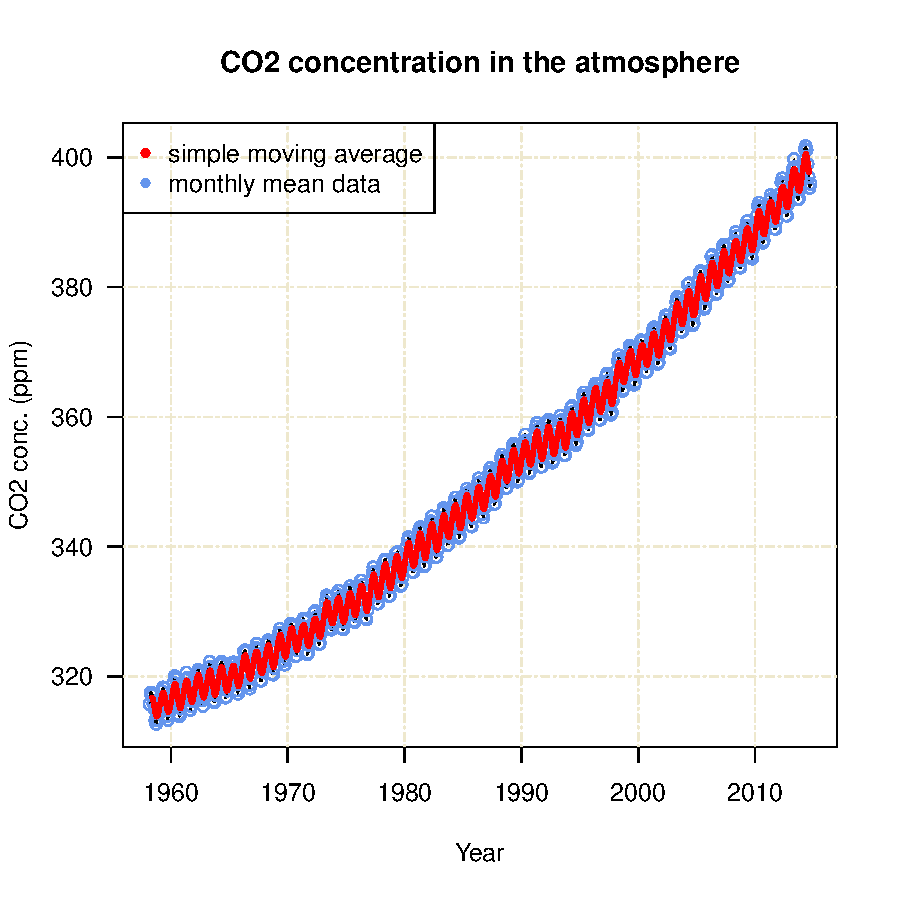
\includegraphics{sweave-fig1visualize}
\caption{Visualization of the CO2 Concentrations}
\end{figure}

The red line in plot \ref{fig1visualize} was computed with a simple moving average. It is not enough to just run a MA.

\section{Decomposition of Time Series}%-----------------------------------------------------------------------------------------------------
A time serie consists of 3 components; a trend component, an irregular (random) component and (if it is a seosonal ts) seasonal component.\\
We can decompose the ts and plot these components:

\begin{figure}
\centering
\begin{Schunk}
\begin{Sinput}
> plot(decompose(yourts)) 
> 
\end{Sinput}
\end{Schunk}
\includegraphics{sweave-decompose}
\caption{Decomposition of the CO2 Time Series}
\end{figure}

It seems that our data can probably be described using an additive model, since the random fluctuations in the data are roughly constant in size over time (constant seasonal component)


\subsection{Decomposing Non-Seasonal Data}%----------------------------------------------------------------------------------------------------

Our example 2 contains the Measurements of the annual flow of the river Nile at Ashwan 1871 \- <U+0080><U+0093>1970. The dataset is in the Package {datasets}. \\
First we visualize our data:
\begin{figure}
\centering
\begin{Schunk}
\begin{Sinput}
> str(Nile)
\end{Sinput}
\begin{Soutput}
 Time-Series [1:100] from 1871 to 1970: 1120 1160 963 1210 1160 1160 813 1230 1370 1140 ...
\end{Soutput}
\begin{Sinput}
> plot(Nile, main="Annual flow of teh Nile", ylab="Flow [V/a]")
\end{Sinput}
\end{Schunk}
\caption{Annual Flow of the Nile}
\end{figure}

A non-seasonal time series consists of a trend and an irregular component. 
To estimate the trend component of a non-seasonal time series that can be described using an additive model, it is common to use a smoothing method, such as calculating the simple moving average of the time series.

The SMA() function in the “TTR” R package can be used to smooth time series data using a simple moving average. 
\begin{figure}
\centering
\begin{Schunk}
\begin{Sinput}
> library(TTR)
> plot(SMA(Nile,n=20))
> 
\end{Sinput}
\end{Schunk}
\includegraphics{sweave-008}
\caption{Trend of the Annual Flow of the Nile}
\end{figure}
We can see that there was a negative trend until 1920 and that it becomes positiv since then. However it is difficult to make a clear statement of the trends, since there are high fluctuations in the data.


Now we can procede plotting the correlograms:
\begin{figure}
\centering
\begin{Schunk}
\begin{Sinput}
> par(mfrow = c(1, 2))
> acf(Nile)
> pacf(Nile)
> par(mfrow = c(1, 1))
\end{Sinput}
\end{Schunk}
\includegraphics{sweave-009}
\caption{Autocorrelations and Partial autocorrelations.}
\end{figure}

We find a significant autocorrelation at the first lags only, that means that the autocorrelation is not constanst over the time.
At the Partial autocorrelation plot we do not observe a significant autocorrelation. 


\subsection{Decomposing Seasonal Data}%----------------------------------------------------------------------------------------------------

We can see each component with:
\begin{Schunk}
\begin{Sinput}
> yourts.components<- decompose(yourts)
\end{Sinput}
\end{Schunk}
\includegraphics{sweave-010}
\begin{Schunk}
\begin{Soutput}
             Jan         Feb         Mar         Apr         May         Jun
1958                          1.44050740  2.56300740  2.99546099  2.31164281
1959  0.04630353  0.67408626  1.44050740  2.56300740  2.99546099  2.31164281
1960  0.04630353  0.67408626  1.44050740  2.56300740  2.99546099  2.31164281
1961  0.04630353  0.67408626  1.44050740  2.56300740  2.99546099  2.31164281
1962  0.04630353  0.67408626  1.44050740  2.56300740  2.99546099  2.31164281
1963  0.04630353  0.67408626  1.44050740  2.56300740  2.99546099  2.31164281
1964  0.04630353  0.67408626  1.44050740  2.56300740  2.99546099  2.31164281
1965  0.04630353  0.67408626  1.44050740  2.56300740  2.99546099  2.31164281
1966  0.04630353  0.67408626  1.44050740  2.56300740  2.99546099  2.31164281
1967  0.04630353  0.67408626  1.44050740  2.56300740  2.99546099  2.31164281
1968  0.04630353  0.67408626  1.44050740  2.56300740  2.99546099  2.31164281
1969  0.04630353  0.67408626  1.44050740  2.56300740  2.99546099  2.31164281
1970  0.04630353  0.67408626  1.44050740  2.56300740  2.99546099  2.31164281
1971  0.04630353  0.67408626  1.44050740  2.56300740  2.99546099  2.31164281
1972  0.04630353  0.67408626  1.44050740  2.56300740  2.99546099  2.31164281
1973  0.04630353  0.67408626  1.44050740  2.56300740  2.99546099  2.31164281
1974  0.04630353  0.67408626  1.44050740  2.56300740  2.99546099  2.31164281
1975  0.04630353  0.67408626  1.44050740  2.56300740  2.99546099  2.31164281
1976  0.04630353  0.67408626  1.44050740  2.56300740  2.99546099  2.31164281
1977  0.04630353  0.67408626  1.44050740  2.56300740  2.99546099  2.31164281
1978  0.04630353  0.67408626  1.44050740  2.56300740  2.99546099  2.31164281
1979  0.04630353  0.67408626  1.44050740  2.56300740  2.99546099  2.31164281
1980  0.04630353  0.67408626  1.44050740  2.56300740  2.99546099  2.31164281
1981  0.04630353  0.67408626  1.44050740  2.56300740  2.99546099  2.31164281
1982  0.04630353  0.67408626  1.44050740  2.56300740  2.99546099  2.31164281
1983  0.04630353  0.67408626  1.44050740  2.56300740  2.99546099  2.31164281
1984  0.04630353  0.67408626  1.44050740  2.56300740  2.99546099  2.31164281
1985  0.04630353  0.67408626  1.44050740  2.56300740  2.99546099  2.31164281
1986  0.04630353  0.67408626  1.44050740  2.56300740  2.99546099  2.31164281
1987  0.04630353  0.67408626  1.44050740  2.56300740  2.99546099  2.31164281
1988  0.04630353  0.67408626  1.44050740  2.56300740  2.99546099  2.31164281
1989  0.04630353  0.67408626  1.44050740  2.56300740  2.99546099  2.31164281
1990  0.04630353  0.67408626  1.44050740  2.56300740  2.99546099  2.31164281
1991  0.04630353  0.67408626  1.44050740  2.56300740  2.99546099  2.31164281
1992  0.04630353  0.67408626  1.44050740  2.56300740  2.99546099  2.31164281
1993  0.04630353  0.67408626  1.44050740  2.56300740  2.99546099  2.31164281
1994  0.04630353  0.67408626  1.44050740  2.56300740  2.99546099  2.31164281
1995  0.04630353  0.67408626  1.44050740  2.56300740  2.99546099  2.31164281
1996  0.04630353  0.67408626  1.44050740  2.56300740  2.99546099  2.31164281
1997  0.04630353  0.67408626  1.44050740  2.56300740  2.99546099  2.31164281
1998  0.04630353  0.67408626  1.44050740  2.56300740  2.99546099  2.31164281
1999  0.04630353  0.67408626  1.44050740  2.56300740  2.99546099  2.31164281
2000  0.04630353  0.67408626  1.44050740  2.56300740  2.99546099  2.31164281
2001  0.04630353  0.67408626  1.44050740  2.56300740  2.99546099  2.31164281
2002  0.04630353  0.67408626  1.44050740  2.56300740  2.99546099  2.31164281
2003  0.04630353  0.67408626  1.44050740  2.56300740  2.99546099  2.31164281
2004  0.04630353  0.67408626  1.44050740  2.56300740  2.99546099  2.31164281
2005  0.04630353  0.67408626  1.44050740  2.56300740  2.99546099  2.31164281
2006  0.04630353  0.67408626  1.44050740  2.56300740  2.99546099  2.31164281
2007  0.04630353  0.67408626  1.44050740  2.56300740  2.99546099  2.31164281
2008  0.04630353  0.67408626  1.44050740  2.56300740  2.99546099  2.31164281
2009  0.04630353  0.67408626  1.44050740  2.56300740  2.99546099  2.31164281
2010  0.04630353  0.67408626  1.44050740  2.56300740  2.99546099  2.31164281
2011  0.04630353  0.67408626  1.44050740  2.56300740  2.99546099  2.31164281
2012  0.04630353  0.67408626  1.44050740  2.56300740  2.99546099  2.31164281
2013  0.04630353  0.67408626  1.44050740  2.56300740  2.99546099  2.31164281
2014  0.04630353  0.67408626  1.44050740  2.56300740  2.99546099  2.31164281
             Jul         Aug         Sep         Oct         Nov         Dec
1958  0.71752160 -1.44085719 -3.10118159 -3.22900897 -2.07282594 -0.90465630
1959  0.71752160 -1.44085719 -3.10118159 -3.22900897 -2.07282594 -0.90465630
1960  0.71752160 -1.44085719 -3.10118159 -3.22900897 -2.07282594 -0.90465630
1961  0.71752160 -1.44085719 -3.10118159 -3.22900897 -2.07282594 -0.90465630
1962  0.71752160 -1.44085719 -3.10118159 -3.22900897 -2.07282594 -0.90465630
1963  0.71752160 -1.44085719 -3.10118159 -3.22900897 -2.07282594 -0.90465630
1964  0.71752160 -1.44085719 -3.10118159 -3.22900897 -2.07282594 -0.90465630
1965  0.71752160 -1.44085719 -3.10118159 -3.22900897 -2.07282594 -0.90465630
1966  0.71752160 -1.44085719 -3.10118159 -3.22900897 -2.07282594 -0.90465630
1967  0.71752160 -1.44085719 -3.10118159 -3.22900897 -2.07282594 -0.90465630
1968  0.71752160 -1.44085719 -3.10118159 -3.22900897 -2.07282594 -0.90465630
1969  0.71752160 -1.44085719 -3.10118159 -3.22900897 -2.07282594 -0.90465630
1970  0.71752160 -1.44085719 -3.10118159 -3.22900897 -2.07282594 -0.90465630
1971  0.71752160 -1.44085719 -3.10118159 -3.22900897 -2.07282594 -0.90465630
1972  0.71752160 -1.44085719 -3.10118159 -3.22900897 -2.07282594 -0.90465630
1973  0.71752160 -1.44085719 -3.10118159 -3.22900897 -2.07282594 -0.90465630
1974  0.71752160 -1.44085719 -3.10118159 -3.22900897 -2.07282594 -0.90465630
1975  0.71752160 -1.44085719 -3.10118159 -3.22900897 -2.07282594 -0.90465630
1976  0.71752160 -1.44085719 -3.10118159 -3.22900897 -2.07282594 -0.90465630
1977  0.71752160 -1.44085719 -3.10118159 -3.22900897 -2.07282594 -0.90465630
1978  0.71752160 -1.44085719 -3.10118159 -3.22900897 -2.07282594 -0.90465630
1979  0.71752160 -1.44085719 -3.10118159 -3.22900897 -2.07282594 -0.90465630
1980  0.71752160 -1.44085719 -3.10118159 -3.22900897 -2.07282594 -0.90465630
1981  0.71752160 -1.44085719 -3.10118159 -3.22900897 -2.07282594 -0.90465630
1982  0.71752160 -1.44085719 -3.10118159 -3.22900897 -2.07282594 -0.90465630
1983  0.71752160 -1.44085719 -3.10118159 -3.22900897 -2.07282594 -0.90465630
1984  0.71752160 -1.44085719 -3.10118159 -3.22900897 -2.07282594 -0.90465630
1985  0.71752160 -1.44085719 -3.10118159 -3.22900897 -2.07282594 -0.90465630
1986  0.71752160 -1.44085719 -3.10118159 -3.22900897 -2.07282594 -0.90465630
1987  0.71752160 -1.44085719 -3.10118159 -3.22900897 -2.07282594 -0.90465630
1988  0.71752160 -1.44085719 -3.10118159 -3.22900897 -2.07282594 -0.90465630
1989  0.71752160 -1.44085719 -3.10118159 -3.22900897 -2.07282594 -0.90465630
1990  0.71752160 -1.44085719 -3.10118159 -3.22900897 -2.07282594 -0.90465630
1991  0.71752160 -1.44085719 -3.10118159 -3.22900897 -2.07282594 -0.90465630
1992  0.71752160 -1.44085719 -3.10118159 -3.22900897 -2.07282594 -0.90465630
1993  0.71752160 -1.44085719 -3.10118159 -3.22900897 -2.07282594 -0.90465630
1994  0.71752160 -1.44085719 -3.10118159 -3.22900897 -2.07282594 -0.90465630
1995  0.71752160 -1.44085719 -3.10118159 -3.22900897 -2.07282594 -0.90465630
1996  0.71752160 -1.44085719 -3.10118159 -3.22900897 -2.07282594 -0.90465630
1997  0.71752160 -1.44085719 -3.10118159 -3.22900897 -2.07282594 -0.90465630
1998  0.71752160 -1.44085719 -3.10118159 -3.22900897 -2.07282594 -0.90465630
1999  0.71752160 -1.44085719 -3.10118159 -3.22900897 -2.07282594 -0.90465630
2000  0.71752160 -1.44085719 -3.10118159 -3.22900897 -2.07282594 -0.90465630
2001  0.71752160 -1.44085719 -3.10118159 -3.22900897 -2.07282594 -0.90465630
2002  0.71752160 -1.44085719 -3.10118159 -3.22900897 -2.07282594 -0.90465630
2003  0.71752160 -1.44085719 -3.10118159 -3.22900897 -2.07282594 -0.90465630
2004  0.71752160 -1.44085719 -3.10118159 -3.22900897 -2.07282594 -0.90465630
2005  0.71752160 -1.44085719 -3.10118159 -3.22900897 -2.07282594 -0.90465630
2006  0.71752160 -1.44085719 -3.10118159 -3.22900897 -2.07282594 -0.90465630
2007  0.71752160 -1.44085719 -3.10118159 -3.22900897 -2.07282594 -0.90465630
2008  0.71752160 -1.44085719 -3.10118159 -3.22900897 -2.07282594 -0.90465630
2009  0.71752160 -1.44085719 -3.10118159 -3.22900897 -2.07282594 -0.90465630
2010  0.71752160 -1.44085719 -3.10118159 -3.22900897 -2.07282594 -0.90465630
2011  0.71752160 -1.44085719 -3.10118159 -3.22900897 -2.07282594 -0.90465630
2012  0.71752160 -1.44085719 -3.10118159 -3.22900897 -2.07282594 -0.90465630
2013  0.71752160 -1.44085719 -3.10118159 -3.22900897 -2.07282594 -0.90465630
2014  0.71752160 -1.44085719 -3.10118159 -3.22900897                        
\end{Soutput}
\end{Schunk}

It seems that our seasonal component is positiv until the sommer months, were it turns to be negativ and turning to be positiv again in the winter

\begin{figure}
\centering
\begin{Schunk}
\begin{Sinput}
> par(mfrow=c(1,2))
> #we can see the trend for the first year:
> ts.plot(yourts.components$seasonal[1:12])
> 
\end{Sinput}
\end{Schunk}
\includegraphics{sweave-decomposition}
\begin{Schunk}
\begin{Sinput}
> ts.plot(aggregate(yourts.components$seasonal))
> #and we can see that this seasonal component is constant over all the years
> 
> yourts.seasonallyadjusted <- yourts - yourts.components$seasonal
> #We can then plot the seasonally adjusted time series using "plot()" 
\end{Sinput}
\end{Schunk}
\includegraphics{sweave-seasonal.component}
\begin{Schunk}
\begin{Sinput}
> plot(yourts, main="TS with seasonal fl.", las=1)
\end{Sinput}
\end{Schunk}
\includegraphics{sweave-seasonallyadjusted}
\begin{Schunk}
\begin{Sinput}
> plot(yourts.seasonallyadjusted, las=1, main="removed seasonal fluctuation")
> par(mfrow=c(1,1))
> 
\end{Sinput}
\end{Schunk}
\includegraphics{sweave-notseasonallyadjusted}
\caption{The seasonal component across the time}
\end{figure}




\section{Forecasts}%----------------------------------------------------------------------------------------------------
We have three different options to make ( up to now)
\begin{enumerate}
  \item predict
  \item Holt Winters
  \item Arima forecasts
\end{enumerate}


\subsection{Forecasting using Exponential Smoothing}%-----------------------------------------------------------------------------------------------

If we have a time series that can be described using an additive model,we can short-time forecast using exponential smoothing.\\
Preconditions:forecast errors are uncorrelated and are normally distributed with mean zero and constant variance.
\begin{Schunk}
\begin{Sinput}
> hw<-HoltWinters(yourts)
> #the alpha value tells us the weight of the previous values for the forecasting
> #values of alpha that are close to 0 mean that little weight is placed on the most recent observations when making forecasts of future values
> #gamma is for the seasonality
> plot(hw)
> 
\end{Sinput}
\end{Schunk}
Holtwinters just makes forecasts for the time period covered by the original data.If we want to forecast for the future, we need the packeged "forecast".

\begin{figure}
\centering
\begin{Schunk}
\begin{Sinput}
> hw1<- forecast.HoltWinters(hw, h=12)
> #for the next year  
> plot.forecast(hw1, main="Prediction for the next year",shadecols = "oldstyle")
> #for next 10 years
> hw10<- forecast.HoltWinters(hw, h=120)
> plot.forecast(hw10, main="Prediction for the next 10 years", shadecols = "oldstyle")
\end{Sinput}
\end{Schunk}
\includegraphics{sweave-017}
\caption{Holt Winters Prediction}
\end{figure}

Here the forecasts for 1913-1920 are plotted as a blue line, the 80% prediction interval as an orange shaded area, and the 95% prediction interval as a yellow shaded area.

The ‘forecast errors’ are calculated as the observed values minus predicted values, for each time point. We can only calculate the forecast errors for the time period covered by our original time series. One measure of the accuracy of the predictive model is the sum-of-squared-errors (SSE) for the in-sample forecast errors.

To calculate a correlogram of the in-sample forecast errors for the CO2 Time series data for lags 1-20, we type:

\begin{figure}
\centering
\begin{Schunk}
\begin{Sinput}
> acf(hw10$residuals, lag.max=20)
\end{Sinput}
\end{Schunk}
\caption{Correlogram of the residuals.}
\end{figure}


\begin{Schunk}
\begin{Sinput}
> Box.test(hw10$residuals, lag=20, type="Ljung-Box")
\end{Sinput}
\begin{Soutput}
	Box-Ljung test

data:  hw10$residuals
X-squared = 37.5445, df = 20, p-value = 0.01006
\end{Soutput}
\end{Schunk}
There is little evidence of non-zero autocorrelations at lags 1-20.

\begin{Schunk}
\begin{Sinput}
> plotForecastErrors <- function(forecasterrors)
+   {
+      # make a histogram of the forecast errors:
+      mybinsize <- IQR(forecasterrors)/4
+      mysd   <- sd(forecasterrors)
+      mymin  <- min(forecasterrors) - mysd*5
+      mymax  <- max(forecasterrors) + mysd*3
+      # generate normally distributed data with mean 0 and standard deviation mysd
+      mynorm <- rnorm(10000, mean=0, sd=mysd)
+      mymin2 <- min(mynorm)
+      mymax2 <- max(mynorm)
+      if (mymin2 < mymin) { mymin <- mymin2 }
+      if (mymax2 > mymax) { mymax <- mymax2 }
+      # make a red histogram of the forecast errors, with the normally distributed data overlaid:
+      mybins <- seq(mymin, mymax, mybinsize)
+      hist(forecasterrors, col="red", freq=FALSE, breaks=mybins)
+      # freq=FALSE ensures the area under the histogram = 1
+      # generate normally distributed data with mean 0 and standard deviation mysd
+      myhist <- hist(mynorm, plot=FALSE, breaks=mybins)
+      # plot the normal curve as a blue line on top of the histogram of forecast errors:
+      points(myhist$mids, myhist$density, type="l", col="blue", lwd=2)
+   }
\end{Sinput}
\end{Schunk}


\begin{figure}
\centering
\begin{Schunk}
\begin{Sinput}
> plotForecastErrors(hw10$residuals)
\end{Sinput}
\end{Schunk}
\caption{Histogram of the errors}
\end{figure}

The histogram of the time series shows that the forecast errors are roughly normally distributed and the mean seems to be close to zero. 


\subsecttion{Seasonal Decomposition of Time Series by Loess}
Forecasting using stl objects:
\begin{figure}
\centering
\begin{Schunk}
\begin{Sinput}
> plot(stlf(yourts, lambda=0, h =120))
> (tslm(yourts~time(yourts)))
\end{Sinput}
\begin{Soutput}
Call:
lm(formula = formula, data = "yourts", na.action = na.exclude)

Coefficients:
 (Intercept)  time(yourts)  
   -2618.494         1.494  
\end{Soutput}
\end{Schunk}
\includegraphics{sweave-022}
\caption{}
\end{figure}

\subsection{ARIMA Models}%-----------------------------------------------------------------------------------------------
For the CO2 time series:
\begin{Schunk}
\begin{Sinput}
> au=auto.arima(yourts, ic = "bic")
> arima1=arima(yourts, order = c(au$arma[1],au$arma[6],au$arma[2]))
> fore1=forecast.Arima(arima1,h=10)
> plot.forecast(fore1)
> 
\end{Sinput}
\end{Schunk}
\includegraphics{sweave-023}

We can first fit an autoregression model to the Nile Time Series:
\begin{figure}
\centering
\begin{Schunk}
\begin{Sinput}
> ar(Nile) # selects order 2
\end{Sinput}
\begin{Soutput}
Call:
ar(x = Nile)

Coefficients:
     1       2  
0.4081  0.1812  

Order selected 2  sigma^2 estimated as  21247
\end{Soutput}
\begin{Sinput}
> cpgram(ar(Nile)$resid)
> arima(Nile, c(2, 0, 0))
\end{Sinput}
\begin{Soutput}
Series: Nile 
ARIMA(2,0,0) with non-zero mean 

Coefficients:
         ar1     ar2  intercept
      0.4096  0.1987   919.8397
s.e.  0.0974  0.0990    35.6410

sigma^2 estimated as 20291:  log likelihood=-637.98
AIC=1283.96   AICc=1284.38   BIC=1294.38
\end{Soutput}
\begin{Sinput}
> 
\end{Sinput}
\end{Schunk}
\includegraphics{sweave-024}
\caption{Cumulative Peridiogram of the residuals}
\end{figure}
Fitting a autoregressive model, we can see that the residuals are well placed.

Structural time series models:
\begin{figure}
\centering
\begin{Schunk}
\begin{Sinput}
> par(mfrow = c(3, 1))
> plot(Nile)
> ## local level model
> (fit <- StructTS(Nile, type = "level"))
\end{Sinput}
\begin{Soutput}
Call:
StructTS(x = Nile, type = "level")

Variances:
  level  epsilon  
   1469    15099  
\end{Soutput}
\begin{Sinput}
> lines(fitted(fit), lty = 2)              # contemporaneous smoothing
> lines(tsSmooth(fit), lty = 2, col = 4)   # fixed-interval smoothing
> plot(residuals(fit)); abline(h = 0, lty = 3)
> ## local trend model
> (fit2 <- StructTS(Nile, type = "trend")) ## constant trend fitted
\end{Sinput}
\begin{Soutput}
Call:
StructTS(x = Nile, type = "trend")

Variances:
  level    slope  epsilon  
   1427        0    15047  
\end{Soutput}
\begin{Sinput}
> pred <- predict(fit, n.ahead = 30)
> ## with 50% confidence interval
> ts.plot(Nile, pred$pred,
+         pred$pred + 0.67*pred$se, pred$pred -0.67*pred$se, col=1:3)
> 
> 
\end{Sinput}
\end{Schunk}
\includegraphics{sweave-025}
\caption{Fitting a Structural Model}
\end{figure}

\subsection{Selecting a Candidate ARIMA Model}%-----------------------------------------------------------------------------------------------


compare both functions of forecasting: 
\begin{Schunk}
\begin{Sinput}
> par(mfrow=c(1,2))
> plot(forecast.arima, xlim=c(2010,2025), ylim=c(385,430))
> plot.forecast(forecasts2 ,xlim=c(2010,2025), ylim=c(385,430))
\end{Sinput}
\end{Schunk}


\section{Links and Further Reading}%-----------------------------------------------------------------------------------------------
\section{Acknowledgements}%------------------------------------------------------------------------------------------------------
Don't forget to thank TeX and R and other opensource communities if you use their products! The correct way to cite R is shown when typing ``\texttt{citation()}'', and ``\texttt{citation("mgcv")}'' for packages.

\clearpage
\end{document}


